\chapter{Background}
\label{chap:background}

In this chapter important theory that is the basis for the proposed design solution in Chapter \ref{chap:design} is presented. R-trees are covered in detail, in addition to different space-filling curves. LSM-trees are also described with challenges that come with its implementation. 

\section{RUM}
The RUM conjecture was introduced in 2016 by Athanassoulis et al\cite{RUM}. It looks at the challenges presented when designing new access methods and the impact it has on read- , write- and memory overhead. The main goal when designing access methods is to minimize read time, update costs and memory usage. Athanassoulis et al classifies the different overheads by these definitions: \newline

\noindent
\textbf{Read Overhead}: The ratio between the total amount of data read including auxiliary (e.g. indexed) and base data, divided by the amount of retrieved data. Also known as \emph{read amplification}.\newline

\noindent
\textbf{Update Overhead}: The ratio between the size of the physical updates performed for one logical update, divided by the size of the logical update. Also known as \emph{write amplification}.\newline

\noindent
\textbf{Memory Overhead}: The ratio between the space utilized for auxiliary and base data, divided by the space utilized for base data. Also known as \emph{space amplification}. \newline

\noindent
The RUM conjecture states that only two of the overheads mentioned above can be prioritized and that this will create a larger overhead for the third. Because of this, it is important to prioritize which overheads to minimize based on the application area. \newline

\noindent
Examples of access methods that prioritize the minimization of read overhead are B+-trees and Skiplists. These methods often implies higher space amplification as additional space is used to store the index structures. \newline

\noindent
In order to minimize update overhead, LSM-trees focuses on being able to load larger bulks of data into storage at once. Write-optimized structures often has an impact on space utilization as there might be empty blocks and data written multiple times. In addition, read access might also suffer as it can be difficult to generate efficient index structures when loading large amounts of data at once.\newline

\noindent
To minimize memory overhead, bloom filters which works as an existence index, could be utilized. This will in turn increase write overhead as compression methods are needed to minimize the storage utilized. It can also increase read overhead as indexes can be sparse and the search is less effective.

\section{R-trees}
R-trees was first presented in 1984 by Antonin Guttman\cite{r-tree} and was created to better handle indexing and retrieval of multidimensional data by their spatial locations. Previous solutions such as B+-trees are not equipped to handle data with multiple dimensions as they only support one-dimensional index structures \cite{ComparisonOfAdvancedTree}. \newline

\noindent
R-trees are structured as a hierarchy with a root node which points to lower nodes until the leaf level nodes are reached. The leaf level nodes contain pointers to the location of where objects are stored. To be able to store multidimensional data objects, R-trees use n-dimensional rectangles to index objects according to a certain space. These rectangles are known as \emph{Minimum Bounding Rectangles} (MBRs) and each root or intermediate node points to the MBRs that is contained within the MBR stored in that node. In the general R-tree, each intermediate node will contain distinct MBRs, even if they are present in several. Each non-leaf node is represented in the tree by (\emph{MBR},  \emph{p}) where \emph{MBR} is the minimum bounding rectangle which spatially contains all MBRs in the child node, and \emph{p} is a pointer to a child node. The leaf-nodes is represented by (\emph{MBR}, \emph{o}) where \emph{MBR} is the minimum bounding rectangle which spatially contains the object, and \emph{o} is the object identifier. The height of the R-tree is at most \(log_mN-1\), when containing N index records. \emph{M} is the maximum number of entries that will fit in one node, and \emph{m} is the minimum number of entries in a node given by \(m <= M/2\). An example of an R-Tree structure can be seen in Figure \ref{fig:RTree} and Figure \ref{fig:RtreeSpace}.

\begin{figure}[ht]
    \centering
    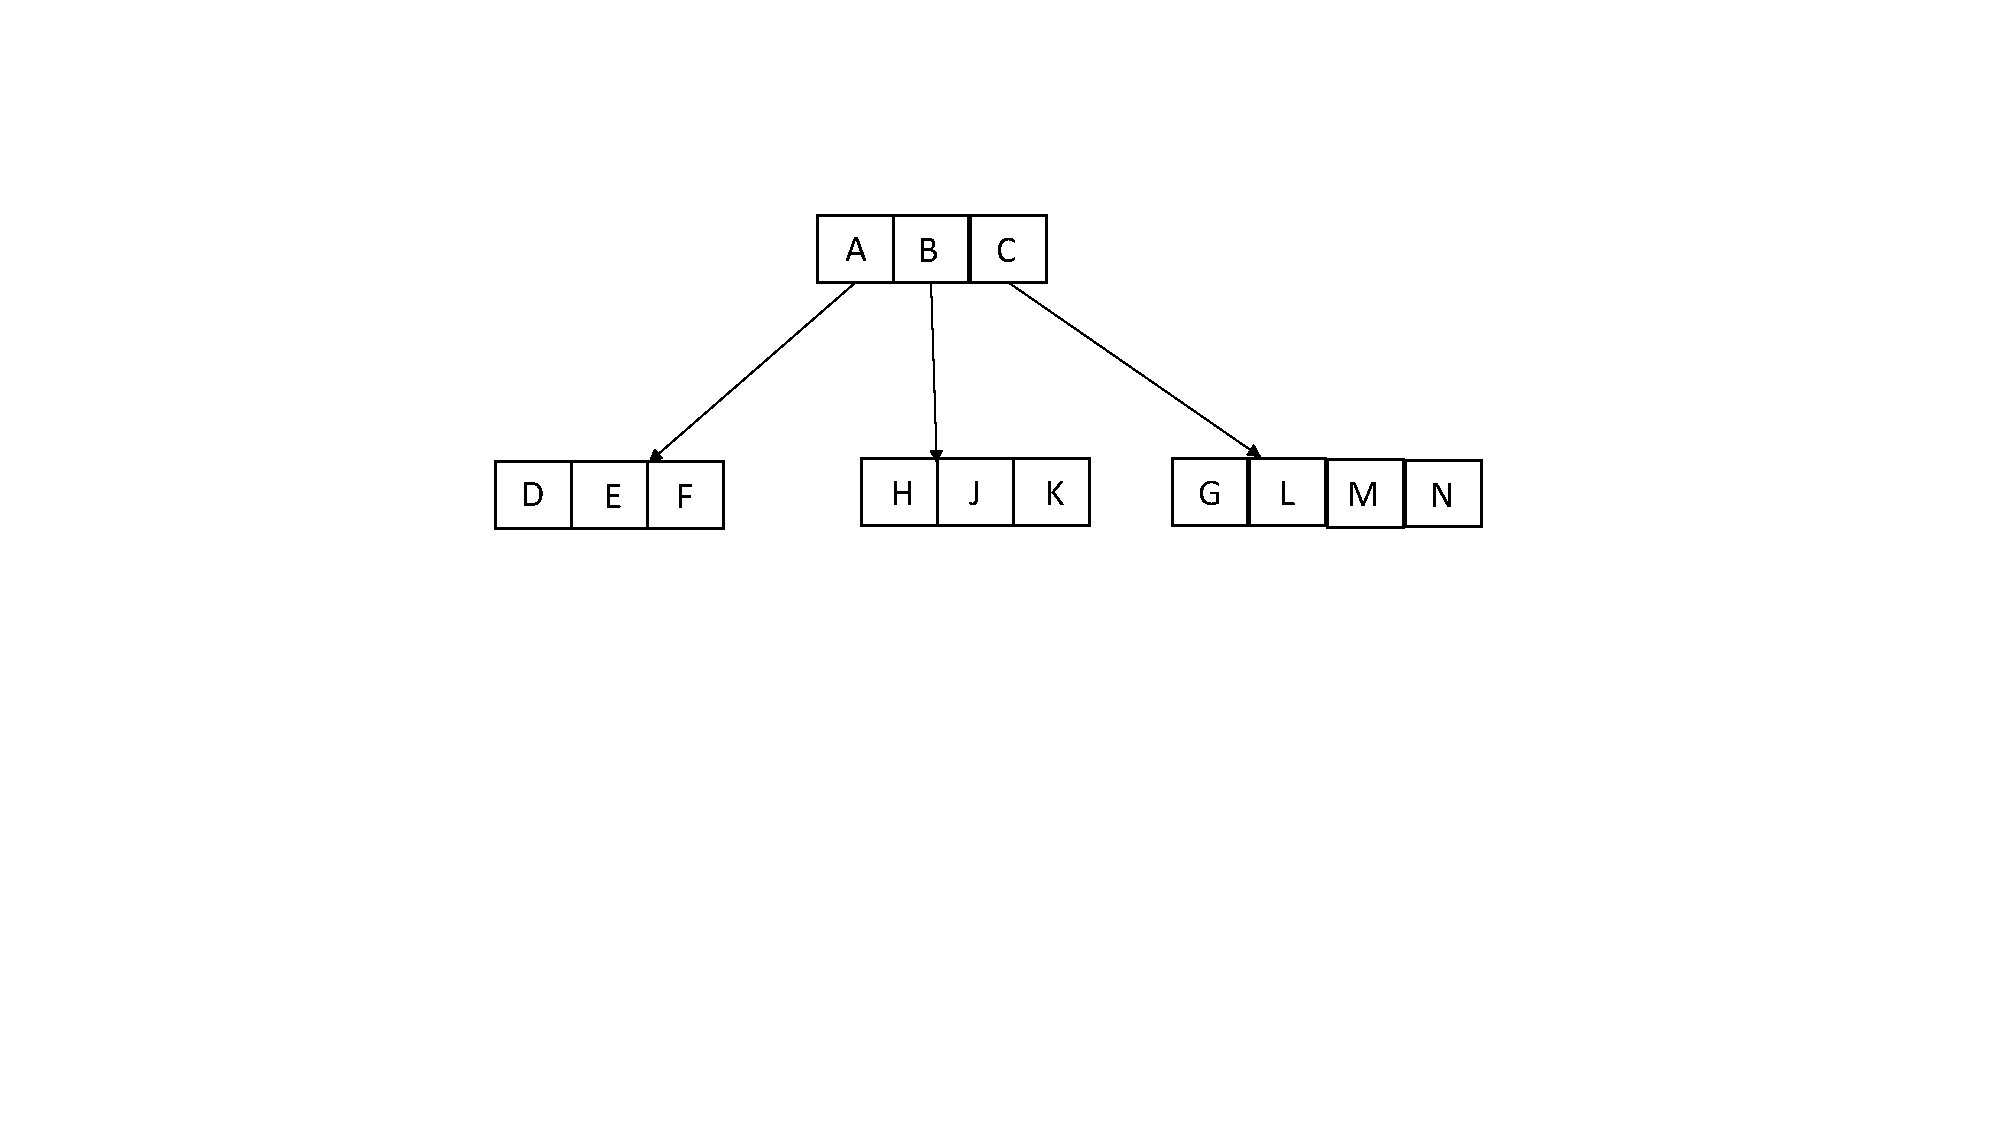
\includegraphics[scale=0.4]{figures/RTree.pdf}
    \caption{R-Tree index structure}
    \label{fig:RTree}
\end{figure}

\begin{figure}[ht]
    \centering
    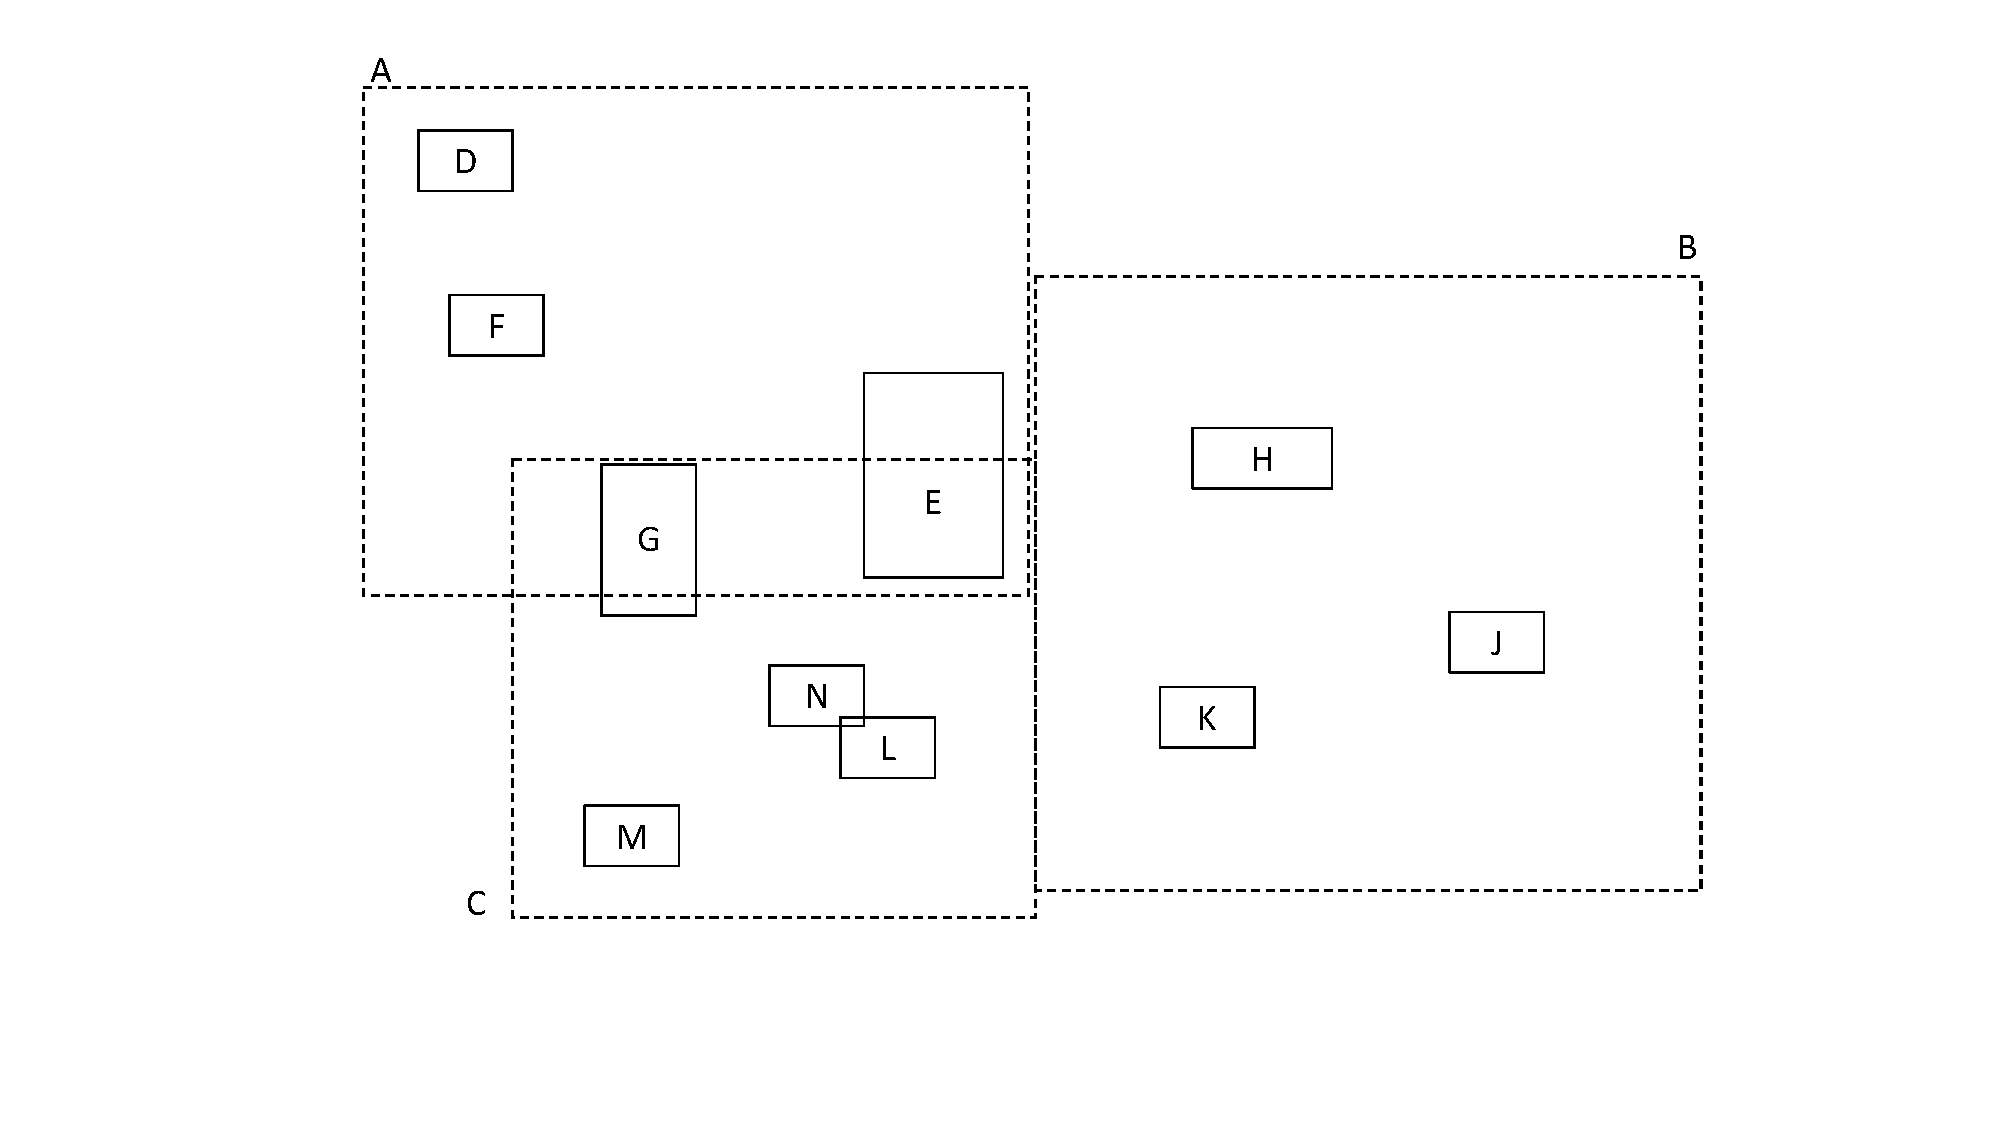
\includegraphics[scale=0.3]{figures/RTree_space.pdf}
    \caption{R-Tree space structure}
    \label{fig:RtreeSpace}
\end{figure}

\subsection{Searching}
Searching in R-trees is done by creating a search rectangle \emph{SR}, and checking all entries in the root node that contains MBRs that overlap with SR. A further search is done by traversing the subtree of the matching entries until all leaf node MBRs that overlap with SR are found. In worst-case scenarios this will lead to the whole tree being searched before finding a match. 

\subsection{Insertion}
Insertions in R-trees are done by inserting the new entry in a leaf node. This is done by searching the tree from the root node and finding the subtrees that overlap with the insertion entry. When the suitable node is found at the leaf level, the entry is placed there as long as the node does not contain the maximum number of entries. If the node is full, which would lead to overflow, the node is split and the tree is adjusted upwards to suit the new index structure. The leaf node which has the least need for area enlargement to fit the new entry is chosen.

\subsection{Deletion}
Deletion is done by first finding the leaf node that contains the entry that is to be deleted. This is done by checking which parts of the tree overlaps with the entry, and when the correct leaf node is found, the entry is removed. After the removal, the remaining leaf node is checked to see if it suffers from node underflow (i.e., contains fewer entries than $m$), and therefore needs readjusting. If this is the case, the tree will be restructured so that each leaf node meets the requirement of having a minimum of \emph{m} entries. 

\subsection{Splitting}
Splitting is a crucial part of working with R-trees as it is used when node overflow occurs, and the choice of splitting method can have a big impact on query performance. An important part of splitting is making as small rectangles as possible for the two new MBRs created by the split. By creating small rectangles, the MBR's are less likely to cover "emtpy" space, which could cause a search to be performed on a subtree, even if this traversal would not yield any search results. In addition, "empty" space in the MBRs could cause worse storage utilization.\newline

\noindent
The splitting methods \emph{Exhaustive Split}, \emph{Quadratic Split} and \emph{Linear Split} was presented by Guttman\cite{r-tree}. In his paper he finds that the linear split method is as good as the more expensive methods without affecting the search performance to an important extent. The quadratic split method is however said to have better overall performance as stated by Beckmann, Kriegel, Schneider and Seeger\cite{R*-tree}.

\subsubsection{Exhaustive Split}
The exhaustive split executes all possible splits and then chooses the split with the MBRs that cover the underlying rectangles with the least "empty" space and smallest overlap. The exhaustive split is the optimal solution, however it is computationally heavy to perform and the number of possible splits is potentially very large.

\subsubsection{Quadratic Split}
The quadratic split is executed by finding the two entries that will create the largest rectangle when combined. Two separate MBRs are then created from each of these entries. The remaining entries are distributed one at a time, by adding it to the MBR that will be enlarged the least. If one of the MBRs will contain less than \emph{m} entries if not all remaining entries are assigned to it, then the remaining points are assigned to that MBR. The cost of this method is quadratic in $M$, as each entry will have to be computed with each other entry when finding the largest space to do the first split. $M$ is the number of entries in a full node. 

\subsubsection{Linear Split}
The linear split is executed similarly as the quadratic split. However, instead of finding the space between each entry, it only finds the distance between the most extreme rectangles. Extreme rectangles are the ones that are the farthest apart on the x-axis. This distance is normalized by taking the width, which is the length between the outer sides of the extreme rectangles. In the end, the pair with the highest value is chosen and put into two new MBRs. The remaining entries are put in the new MBR that require the least enlargement. The cost of this method is linear in $M$. 

\subsection{R+-tree}
The R+-tree is a variant of the general R-tree and was introduced in 1987 by Sellis, Roussopoulos and Faloutsos\cite{R+Tree}. It was developed to avoid overlapping MBRs in intermediate nodes. In the general R-tree each intermediate node contains MBRs which completely covers the MBRs in the child nodes. This can lead to all nodes having to be searched for a specific data object, which is not optimal. To reduce the number of intermediate nodes to be searched, the R+-tree splits the MBRs in intermediate nodes which point to leaf nodes. This is done so these MBRs do not overlap, and instead the MBRs at leaf level can be stored in multiple nodes. An important thing to note however is that the improved search performance of R+-trees has a negative effect on the space utilization. This is however minimal if search performance is an important factor in the use of the R-tree index. The R-tree structure shown in Figure \ref{fig:RTree} and Figure \ref{fig:RtreeSpace} are presented as an R+-structure in Figure \ref{fig:RplusTree} and Figure \ref{fig:RplusTreeSpace}. Notice that node $E$ is now stored in leaf nodes pointed to by both $A$ and the newly created node $O$, while node $G$ has been moved to node $O$. 

\begin{figure}[ht]
    \centering
    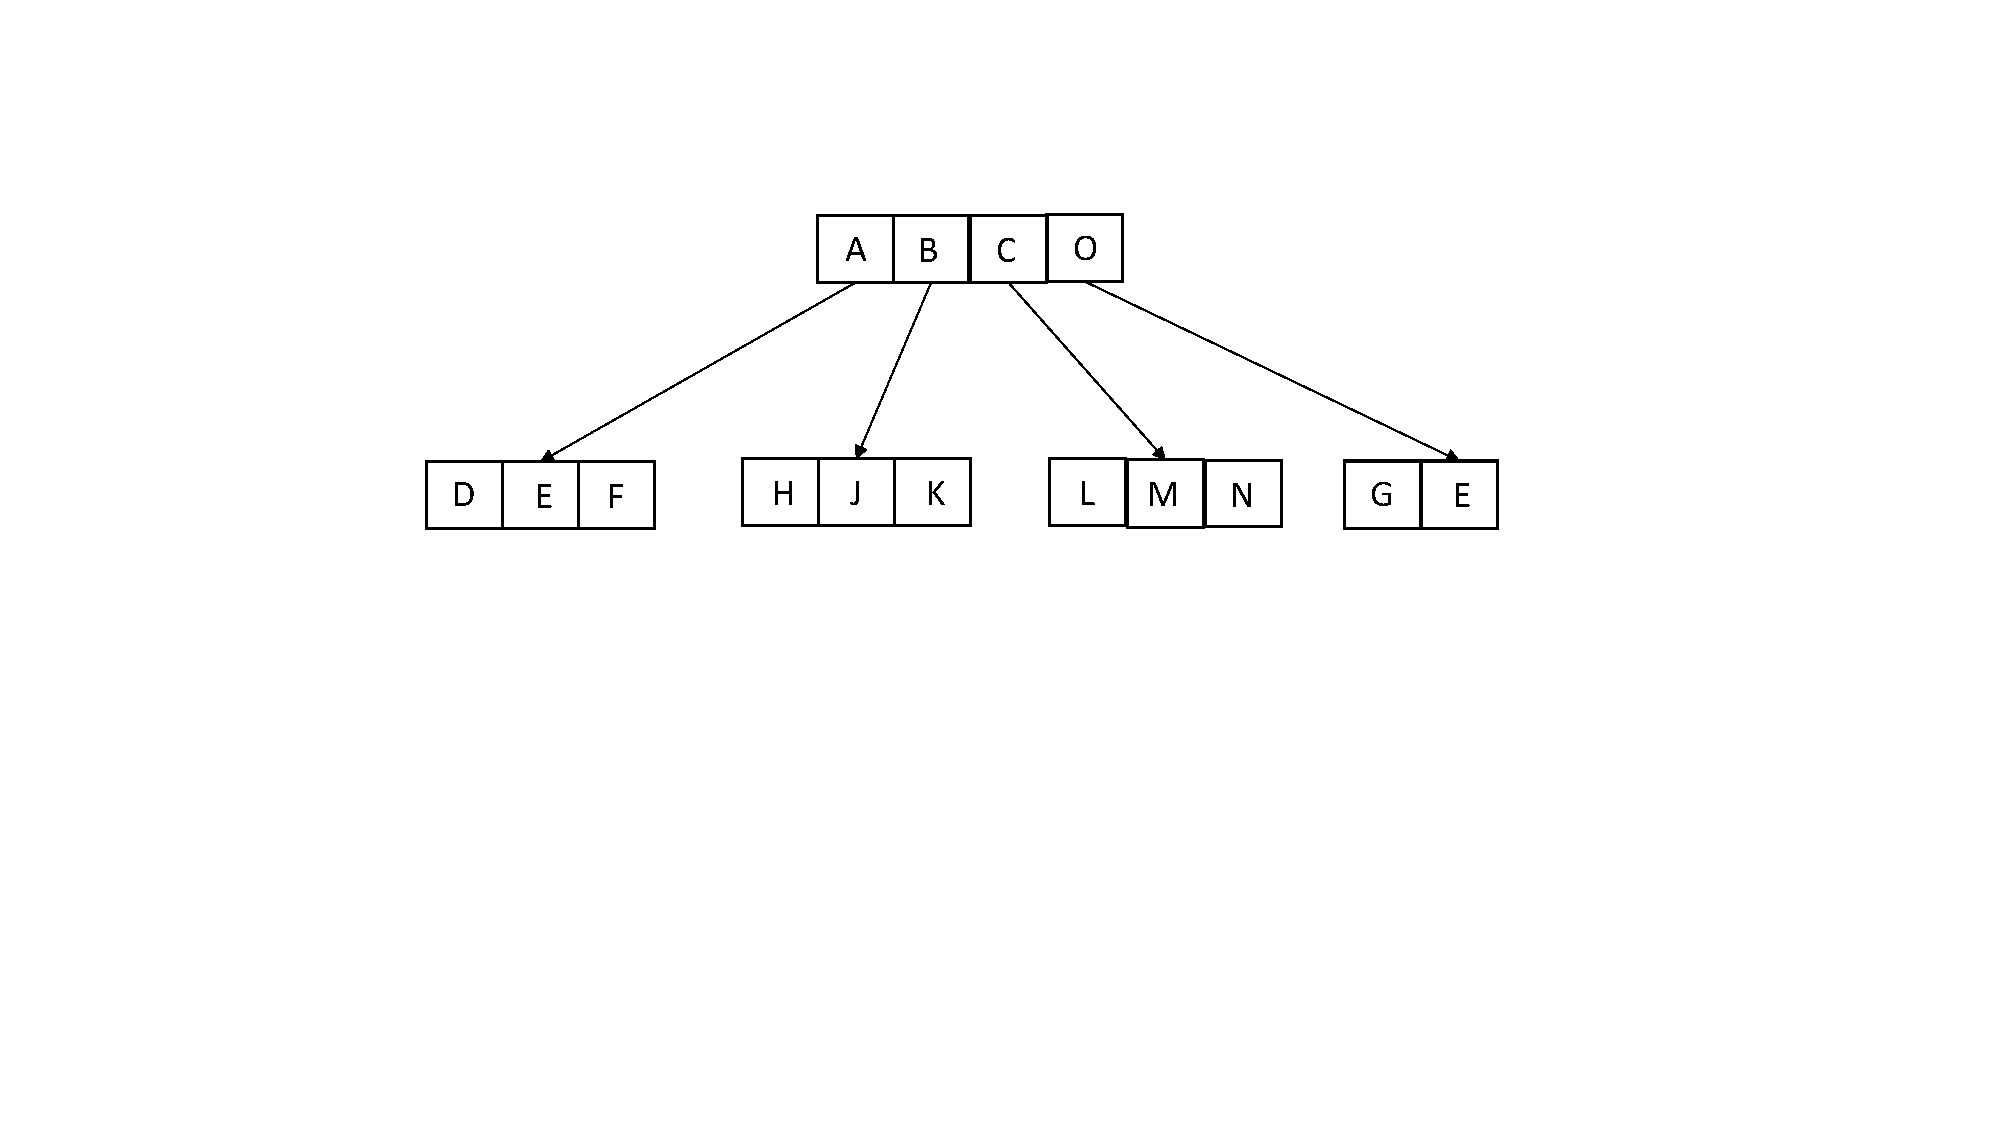
\includegraphics[scale=0.4]{figures/RPlusTree.pdf}
    \caption{R+-Tree index structure}
    \label{fig:RplusTree}
\end{figure}

\begin{figure}[ht]
    \centering
    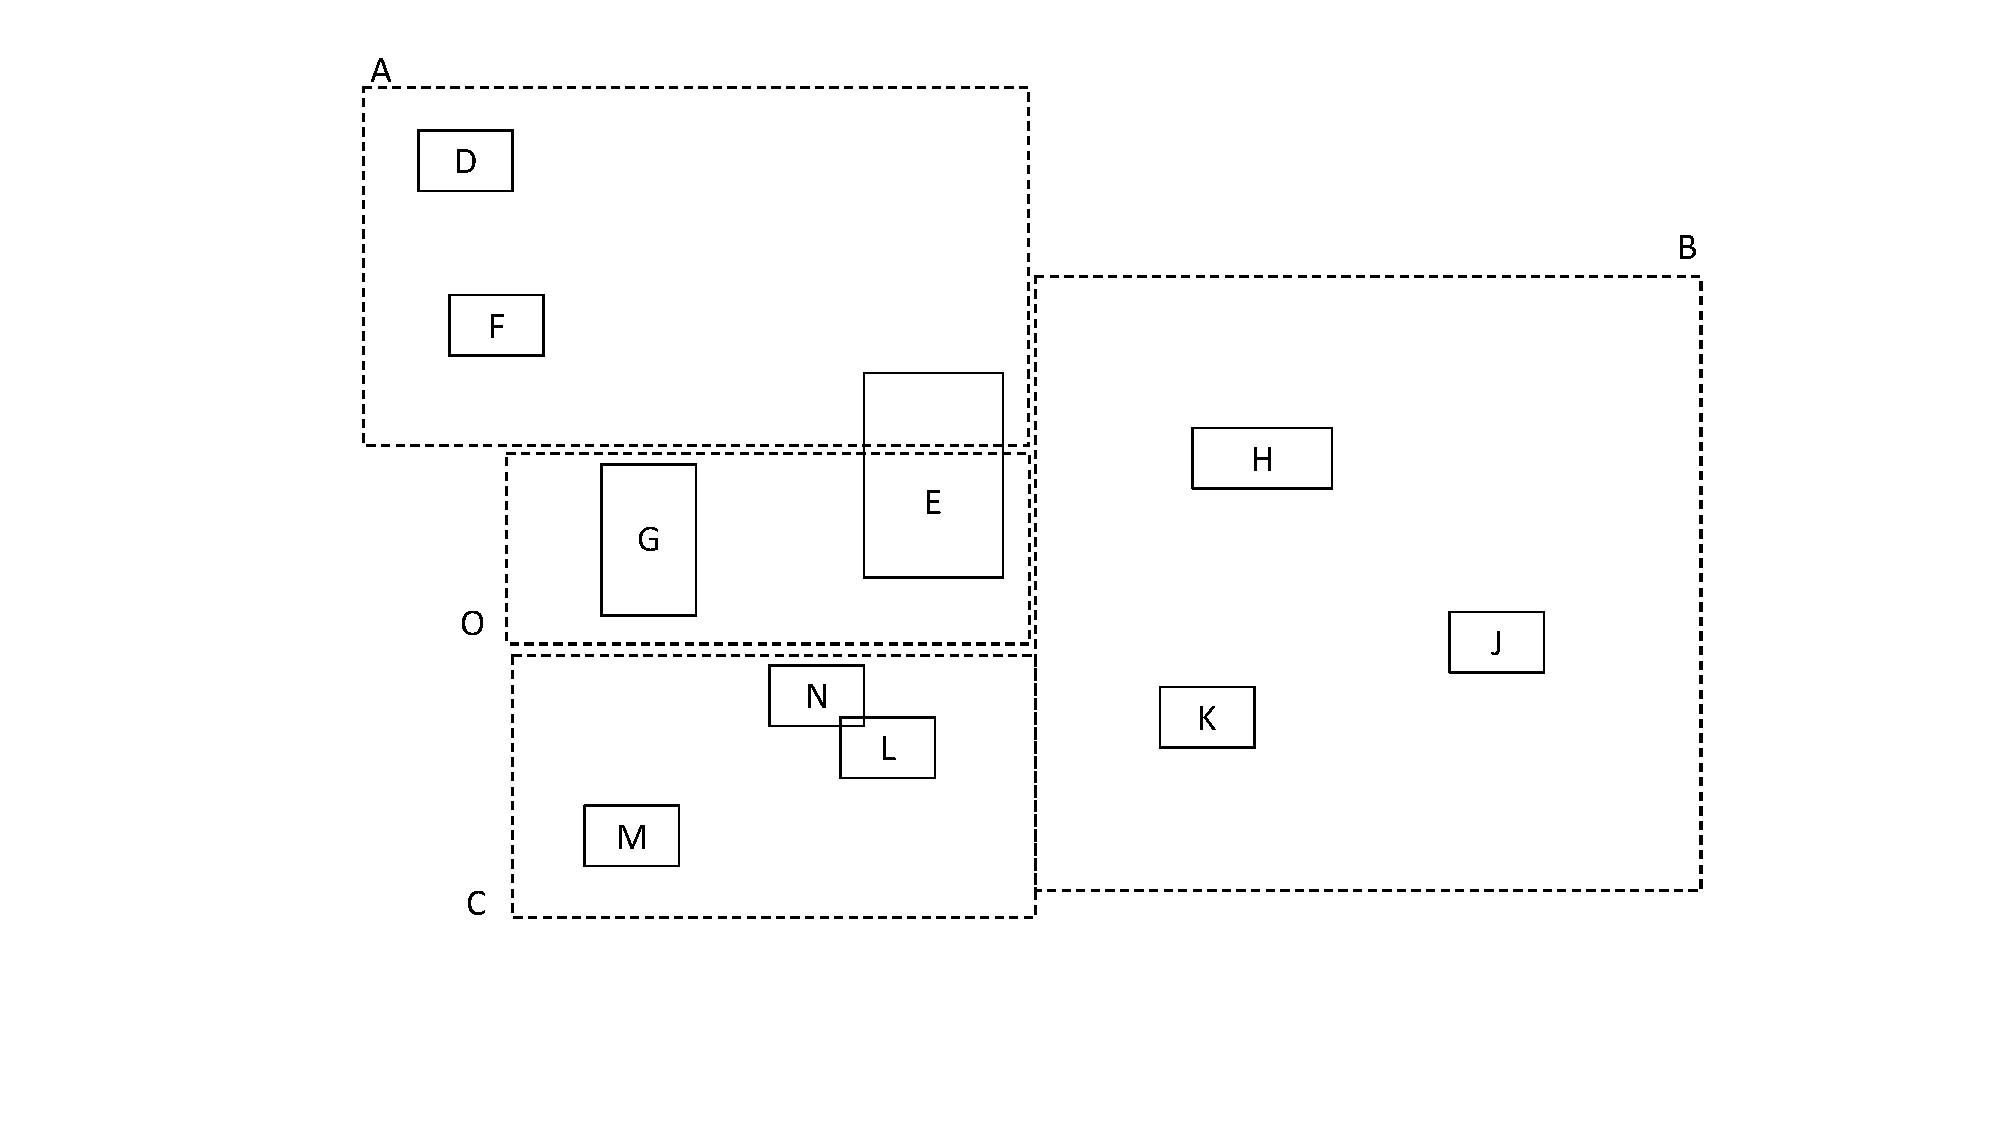
\includegraphics[scale=0.35]{figures/RPlusTree_space.pdf}
    \caption{R+-Tree space structure}
    \label{fig:RplusTreeSpace}
\end{figure}

\subsection{R*-tree}
The R*-tree is an extension of the general R-tree which is attractive as it supports both point and spatial data without increasing the implementation cost too much. This structure was presented in 1990 by Beckmann, Kriegel, Schneider and Seeger\cite{R*-tree}, where different parts that are essential for performance is discussed.\newline

\noindent
\textbf{The area covered by intermediate MBRs should be minimized}\newline
The "empty" space covered by minimum bounding rectangles should be minimized to avoid additional access paths when conducting a search. \newline

\noindent
\textbf{The overlap between intermediate MBRs should be minimized}\newline
When minimizing the overlap, the possible access paths during a search is also minimized. \newline

\noindent
\textbf{The margin of intermediate MBRs should be minimized}\newline
The margin of a minimum bounding rectangle is the sum of each side of the rectangle. Minimization of the margin will lead to more quadratic shaped rectangles, which in turn are easier to place in space without causing overlap. This will again make it easier for the parent MBRs to reduce their size. \newline

\noindent
\textbf{Storage utilization should be optimized}\newline
With higher storage utilization, the height of the tree will be reduced which will lead to lower query costs. \newline

\noindent
An important thing to note is that it is difficult to achieve high storage utilization when also minimizing the area covered by each MBR and their overlap. This is because the shape of the rectangles and the number of entries in each node needs to be more adjustable. Reducing the margin will however most likely lead to better storage utilisation. \newline

\noindent
In order to improve the retrieval performance, the R*-tree focuses on the insertion of new rectangles. When choosing the subtree for insertion, the structure focuses on finding the path which leads to the least need for \emph{overlap} enlargement to include the new entry. This is in contrast to the general R-tree where it decides based on the least need for \emph{area} enlargement in total. If a leaf node is full, the algorithm uses reinsertion if it is the first time a node overflow occurs at that particular level in the tree. Reinsertion is costly, but gives better query performance than node splitting. If a reinsertion has already been used on a level, a splitting method is applied. The splitting method consists of deciding a split axis among all dimensions and choosing the division of entries that lead to the least overlap between the resulting MBRs.

\section{Space-Filling Curves}
Space-Filling Curves (SFCs) were discovered over a hundred years ago by Peano\cite{peano} and  later developed by others such as Hilbert\cite{hilbert}. SFCs are used for mapping data from multidimensional to a one-dimensional space by imposing a linear order on them, while maintaining the position of the data in the space. There are two different objectives when using space-filling curves\cite{IrregularSpace}. \emph{Locality-preserving}, which keeps points that are close in proximity in the multidimensional space close also in the one-dimensional space. And \emph{Order-preserving}, which maintains the order from a specific dimension in the one-dimensional space. The locality-preserving SFCs are good to use in applications that are cluster-based, while the order-preserving SFCs are suited for applications which use some type of sorting, ordering or indexing. \newline

\noindent
The motivation for using space-filling curves in computer related applications is the continuous growth of multidimensional data generated such as multimedia and geographical data. In order to store and query this data efficiently it is crucial that it is possible to order the items so that it can be located in an index structure. The most mentioned space-filling curves with regard to R-trees are the \emph{Z-order curve} and the \emph{Hilbert curve}. \newline

\noindent
The Z-order curve structure for the first three iterations can be seen in Figure \ref{fig:zorder}. Z-order is often also referred to as Morton Code, Peano curve, bit-interleaving or bit-shuffling\cite{performanceSFC}\cite{fractKeyRetri}. The advantage of Z-order is that it is simple and not too costly to implement, in comparison to the Hilbert curve which is both more complex and has a higher computational cost. The structure of the Hilbert curve is shown in Figure \ref{fig:hilbertcurve}, and shows that it rotates its structure through the iterations. It has been shown that the Hilbert curve obtains a better clustering than Z-ordering\cite{AnalysisHilbert}\cite{fractKeyRetri}, which is desirable as it in turn may require less disk accesses during search. 

\begin{figure}[ht]
     \centering
     \begin{subfigure}{0.2\textwidth}
         \centering
         
\includegraphics[width=\textwidth]{figures/spaceFilling_z_1.pdf}
         \caption{Iteration 1}
     \end{subfigure}
     \hfill
      \begin{subfigure}{0.2\textwidth}
     \centering
     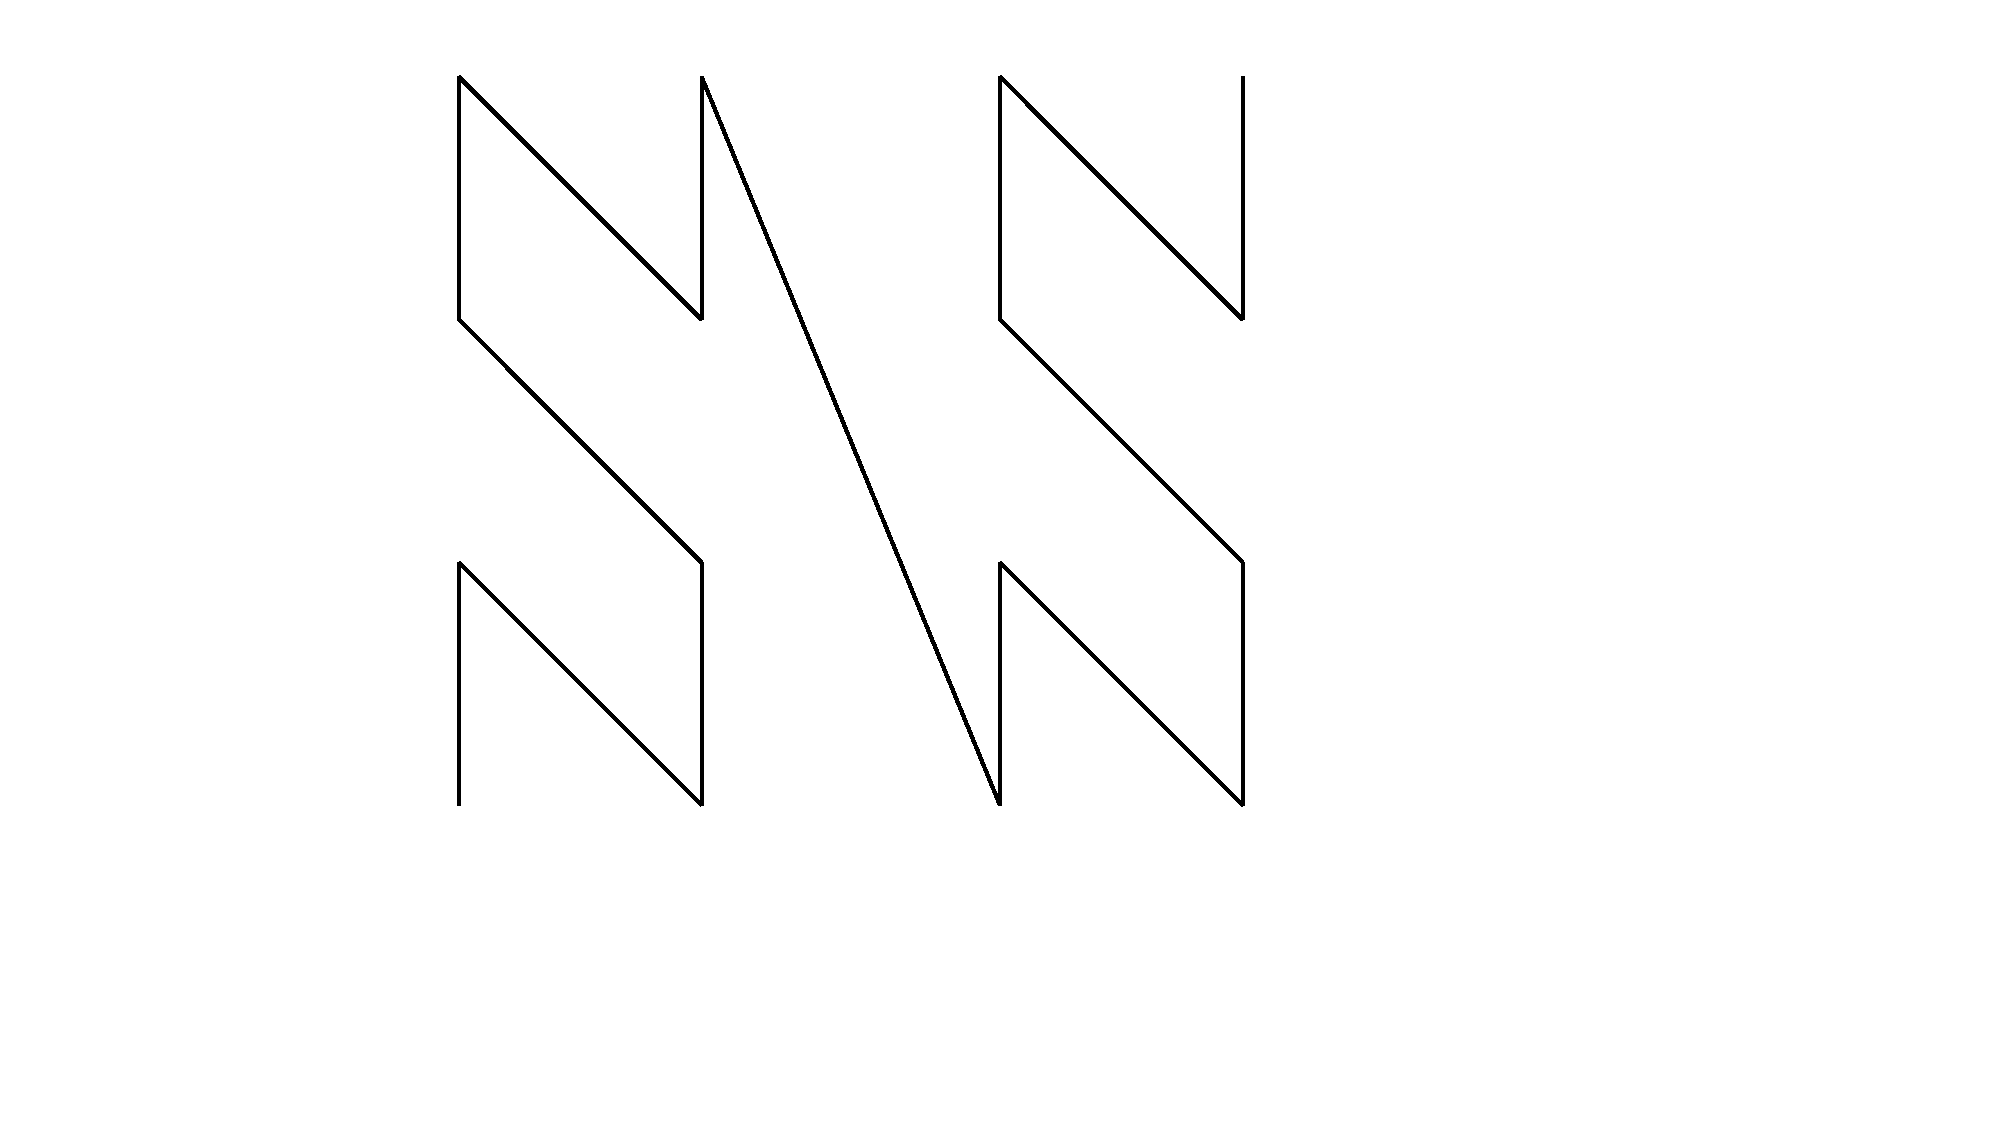
\includegraphics[width=\textwidth]{figures/spaceFilling_z_2.pdf}
     \caption{Iteration 2}
     \end{subfigure}
    \hfill
     \begin{subfigure}{0.2\textwidth}
         \centering
         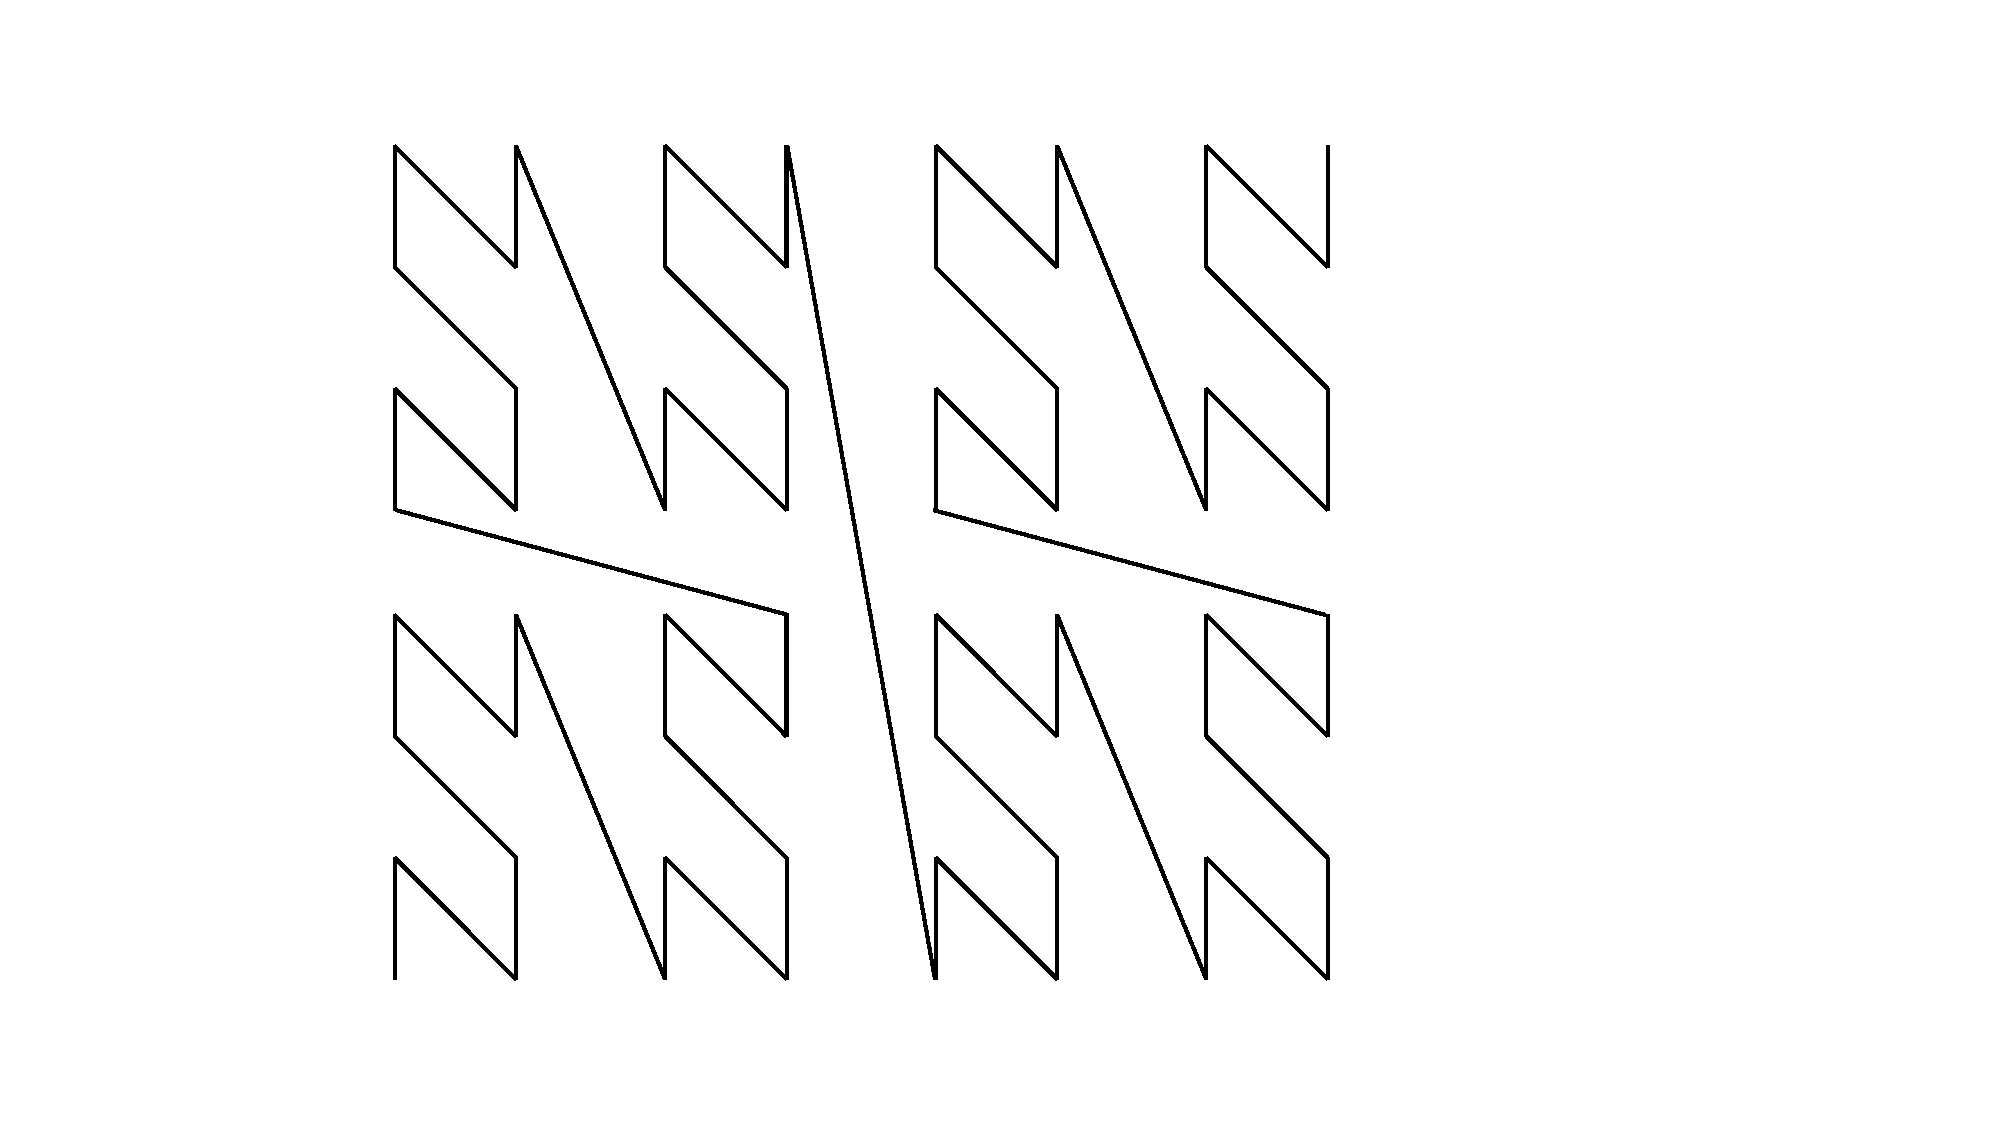
\includegraphics[width=\textwidth]{figures/spaceFilling_z_3.pdf}
         \caption{Iteration 3}
     \end{subfigure}
        \caption{Z-order curve, first three iterations}
        \label{fig:zorder}
\end{figure}

\begin{figure}[ht]
     \centering
     \begin{subfigure}{0.2\textwidth}
         \centering
         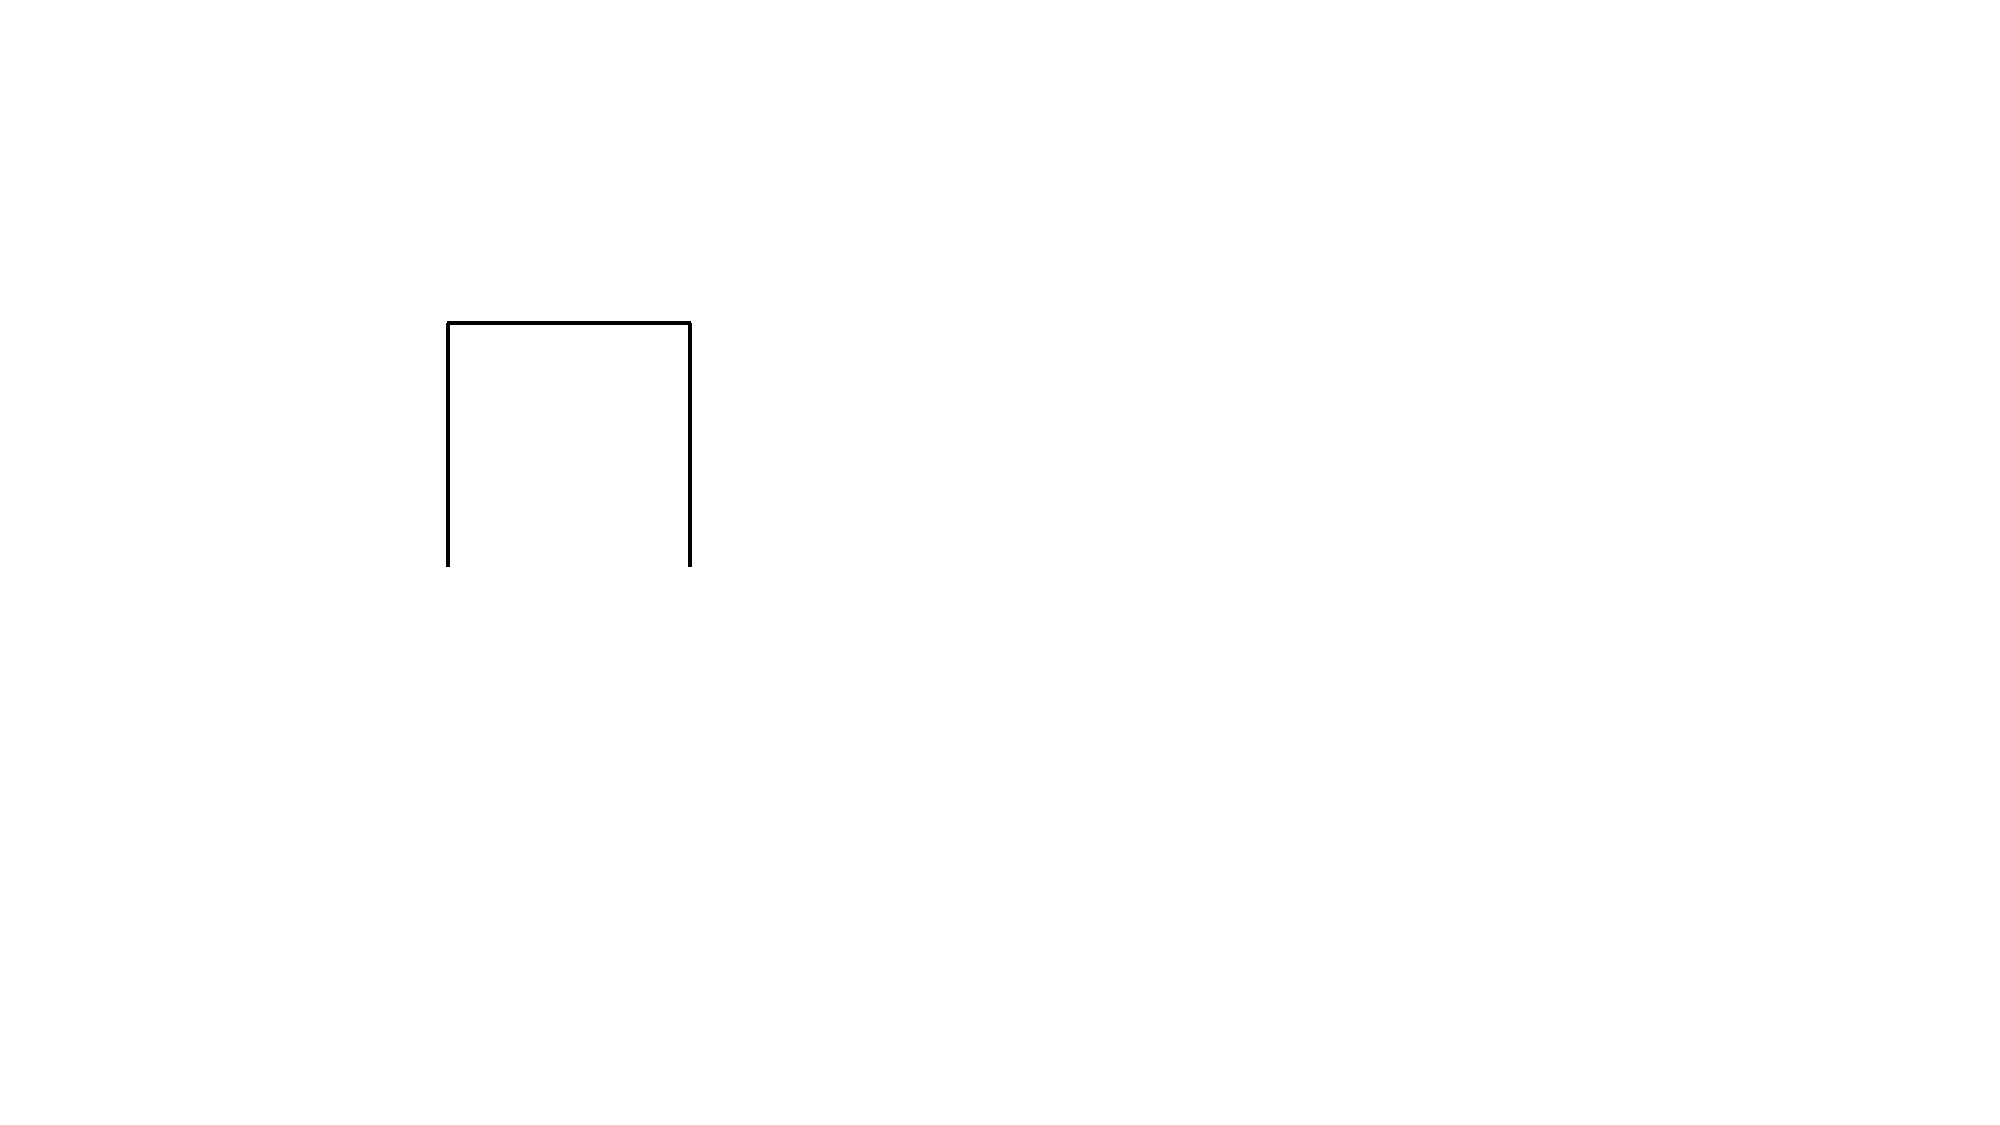
\includegraphics[width=\textwidth]{figures/spaceFilling_h_1.pdf}
         \caption{Iteration 1}
     \end{subfigure}
     \hfill
      \begin{subfigure}{0.2\textwidth}
     \centering
     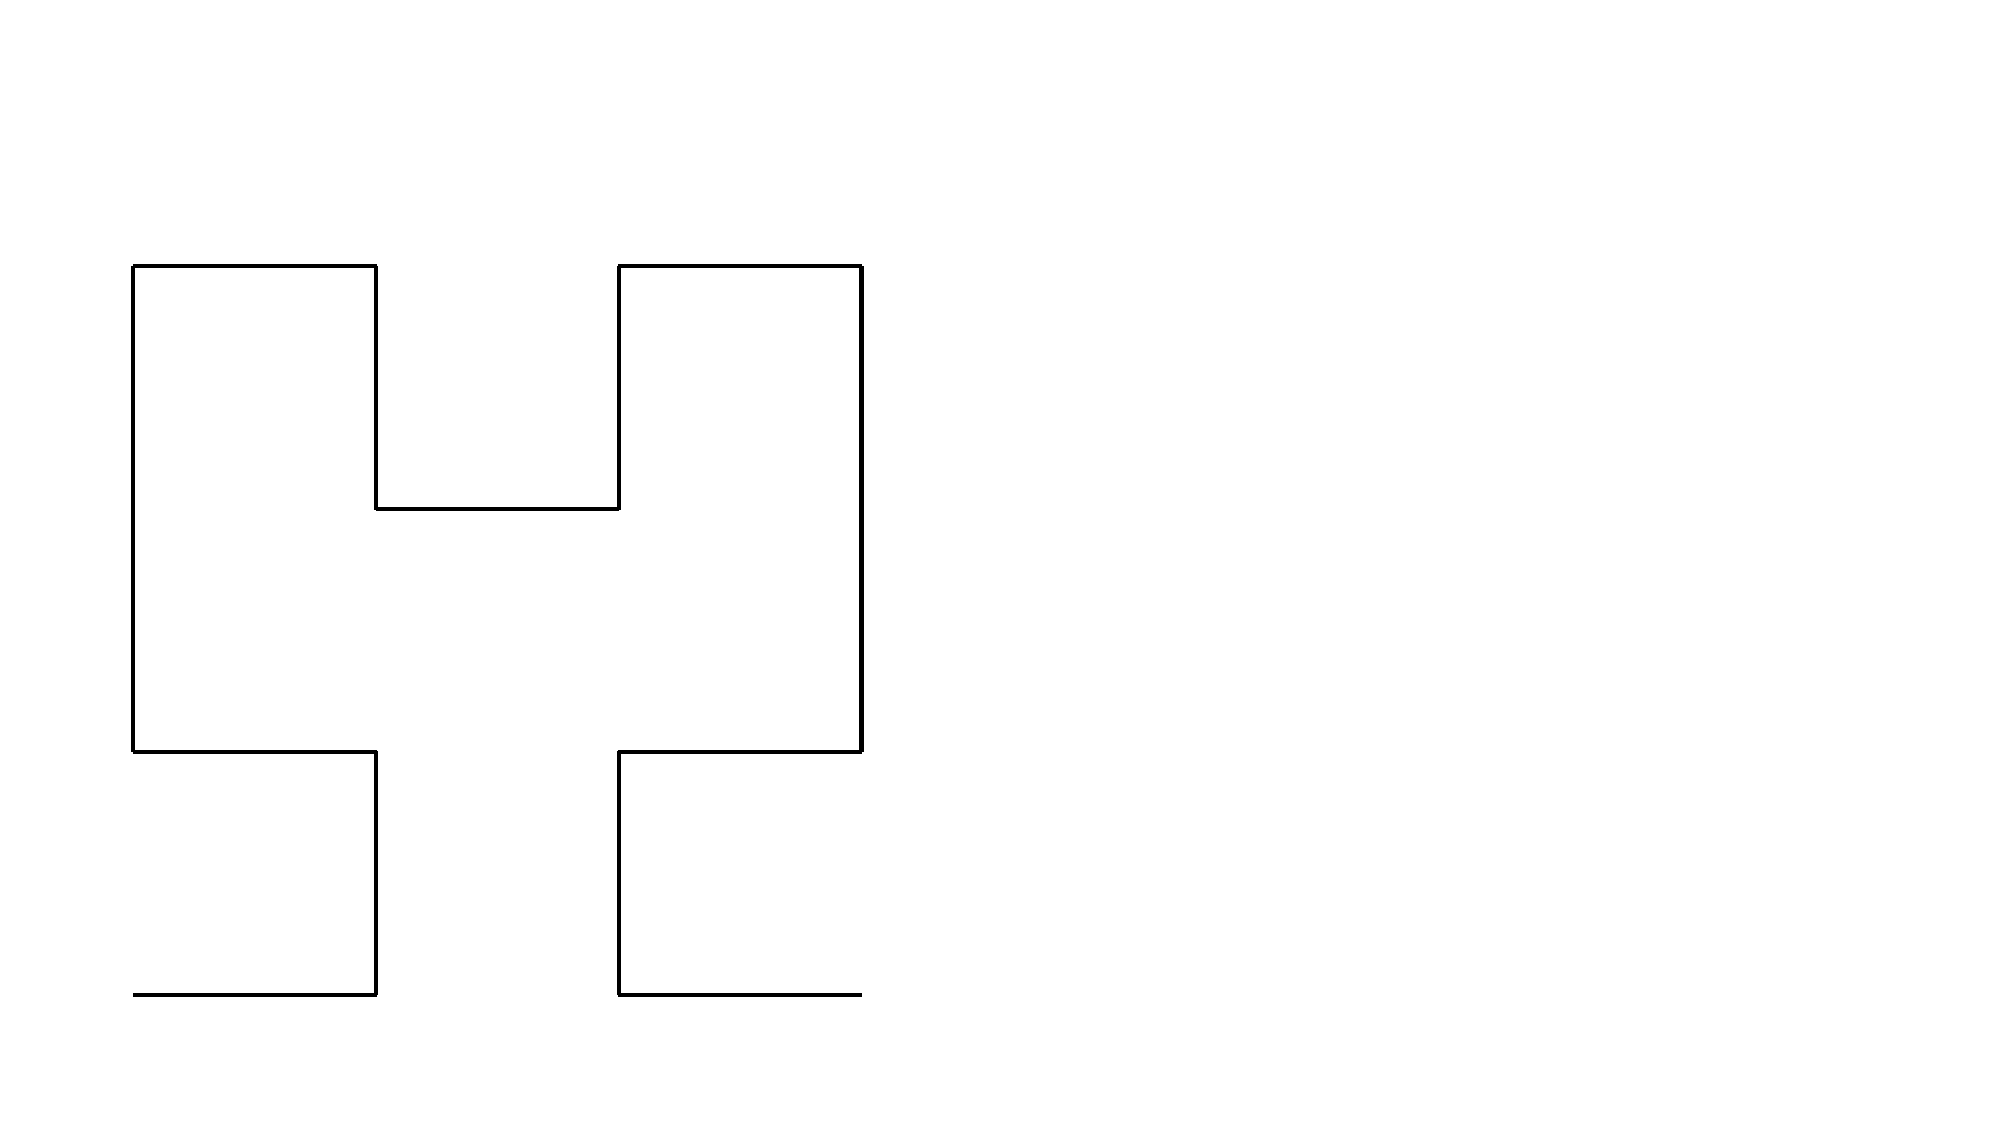
\includegraphics[width=\textwidth]{figures/spaceFilling_h_2.pdf}
     \caption{Iteration 2}
     \end{subfigure}
    \hfill
     \begin{subfigure}{0.2\textwidth}
         \centering
         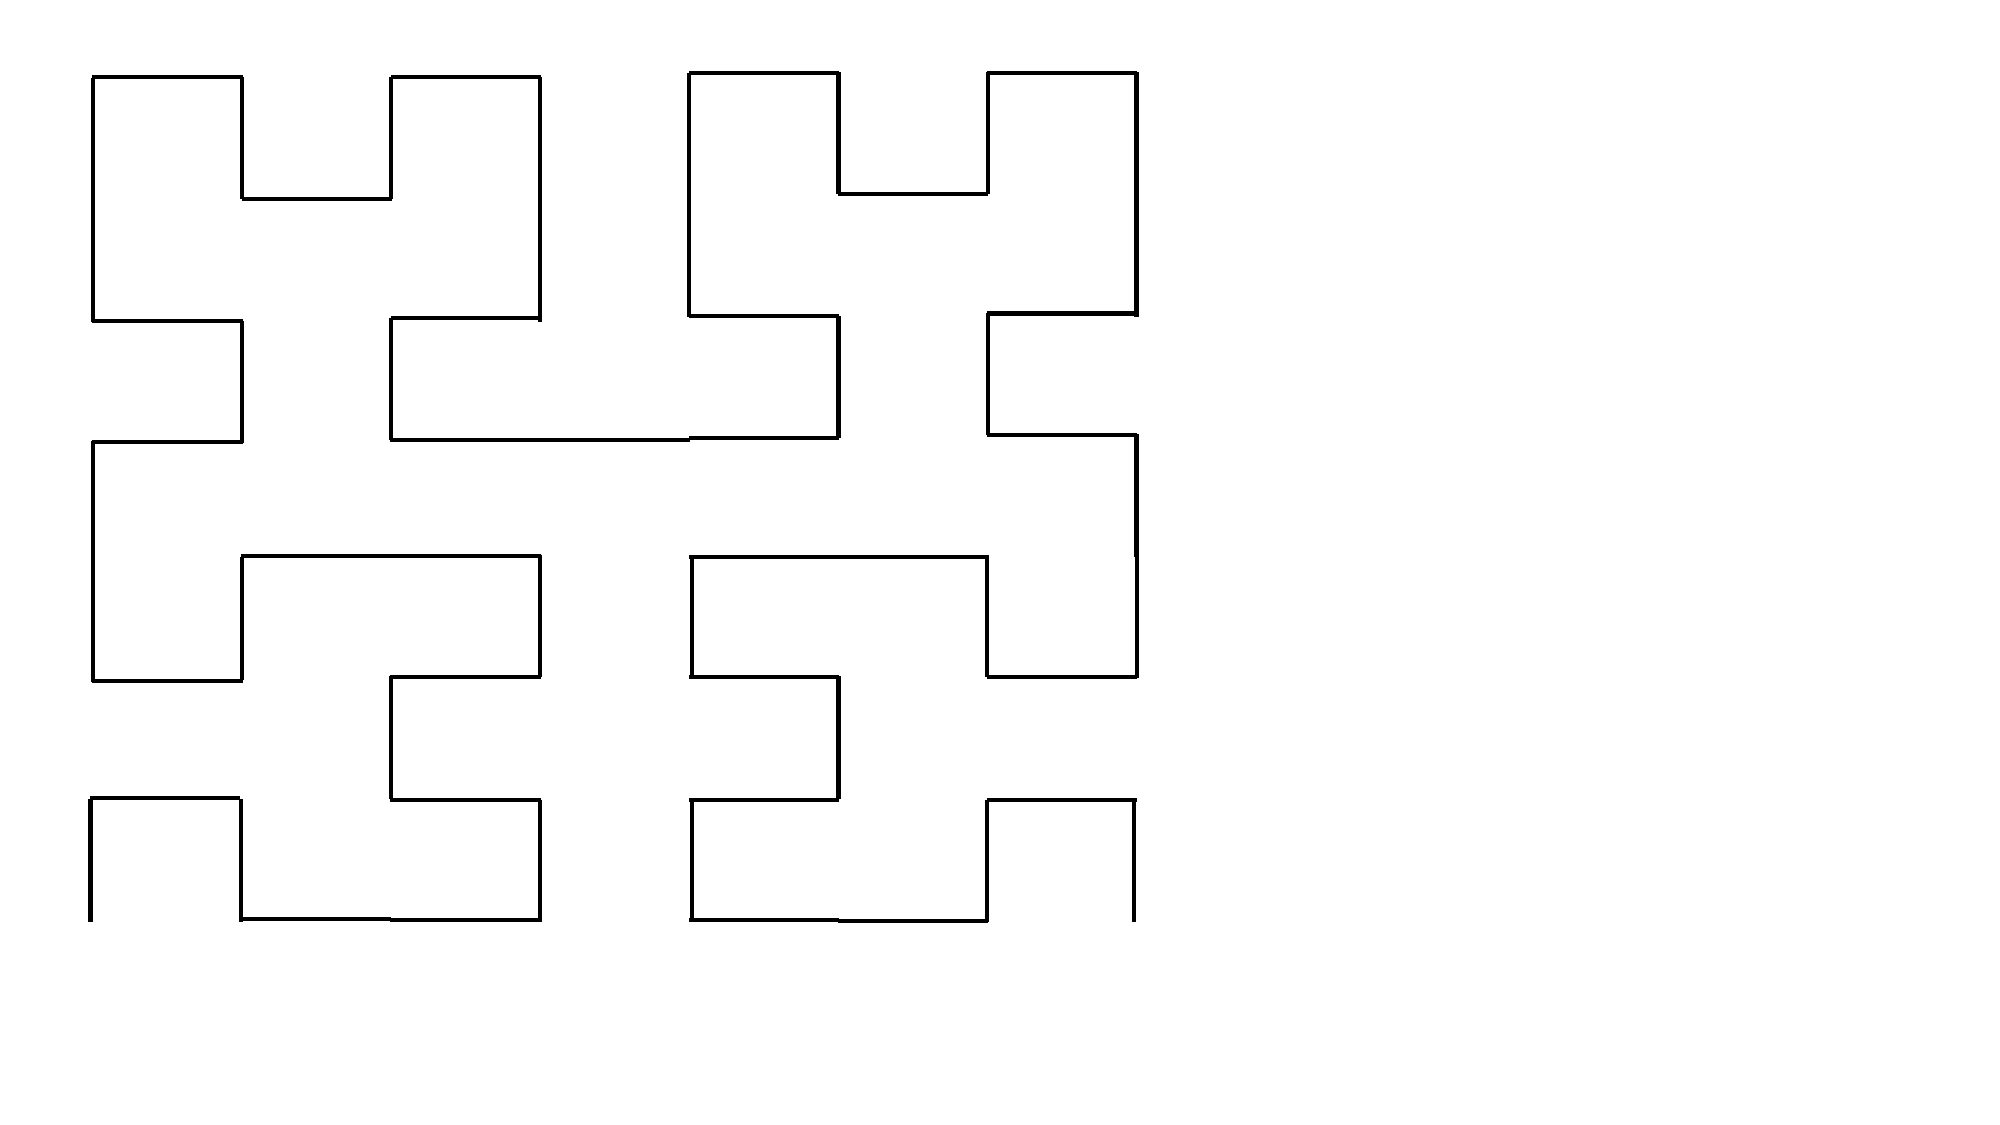
\includegraphics[width=\textwidth]{figures/spaceFilling_h_3.pdf}
         \caption{Iteration 3}
     \end{subfigure}
        \caption{Hilbert curve, first three iterations}
        \label{fig:hilbertcurve}
\end{figure}

\noindent
The main challenge when mapping multidimensional data is maintaining the order of the objects across dimensions. In an ideal space-filling curve the ordering of the data should be the same in every dimension, this is however often not possible to achieve. The use of the application is therefore an important aspect of choosing the best suited space-filling curve. The Z-order curve is the ordering that gives the best mapping across dimensions, when the number of dimensions is low. With the increase of dimensions, the Hilbert curve gets more optimal\cite{IrregularSpace}. This means that with a high level of dimensions, where all dimensions are equally important, the Hilbert curve should be chosen as it is able to maintain a better level of fairness across dimensions. If dimensions can be prioritized, or if there exists a lower level of dimensions, the Z-order curve will be the better choice.

\section{The Log-Structured Merge-Tree}
The \emph{Log-Structured Merge-tree} was introduced in 1996 by O'Neil et al\cite{LSMTree}. It is a write-optimized storage structure created to handle big amounts of insertions, while still being able to search for entries by index. The structure of LSM-trees consists of multiple levels. The top level is in memory, known as $C_0$, where entries are stored in a tree by index. The lower levels $C_1, C_2 ... C_n$ are stored on disk and store its entries in a B-tree like index structure. Instead of inserting one entry at a time, the LSM-tree loads entries to disk in batches by using a method called \emph{rolling merge}. The in-memory component $C_0$ is smaller than the lower components, while the lower components grow in size the further down they are in the chain. When $C_0$ reaches a treshold close to its maximum size, entries are sent to merge with $C_1$ while a batch of entries from $C_1$ are put in a buffer. The block containing the old entries from $C_1$ before merge is called the \emph{emptying} block, while the new leaf nodes merged from $C_0$ is called the \emph{filling} block. The filling block is stored on a new disk page, so the old entries are stored in case recovery is needed. This means that write operations are done in-place in $C_0$, while they are done out-of-place in the lower components. The structure of LSM-trees with two levels can be seen in Figure \ref{fig:LSMTree}, while the rolling merge process can be seen in Figure \ref{fig:LSMMerge}. 

\begin{figure}[ht]
    \centering
    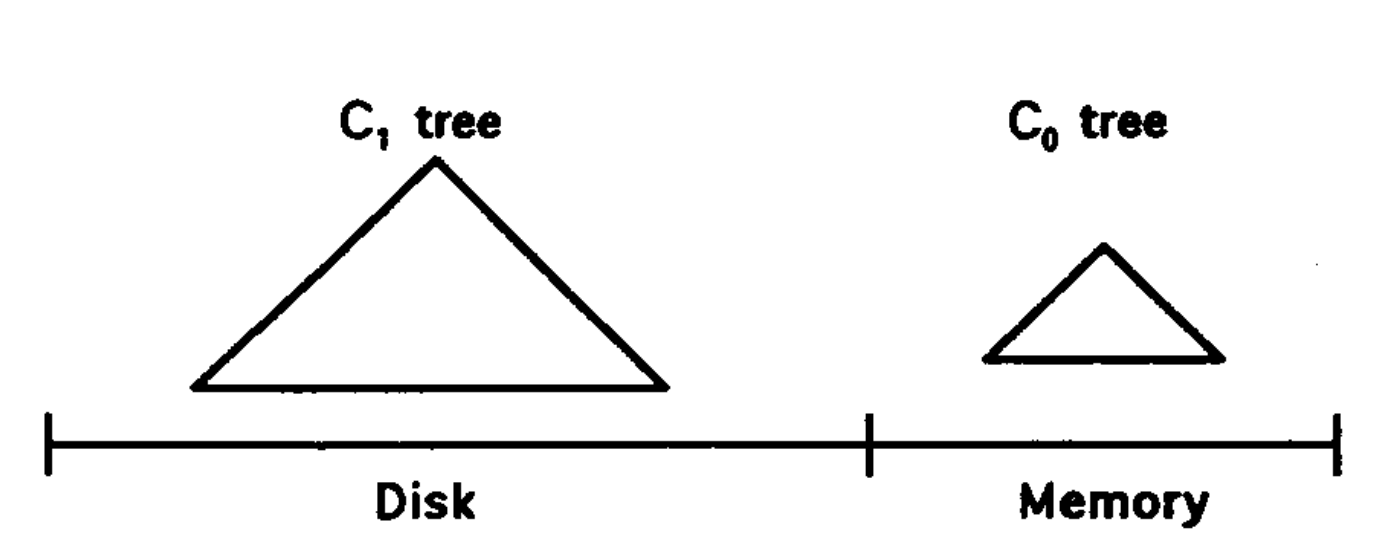
\includegraphics[scale=0.3]{figures/LSM.png}
    \caption{LSM-tree with two levels\cite{LSMTree}}
    \label{fig:LSMTree}
\end{figure}

\begin{figure}[ht]
    \centering
    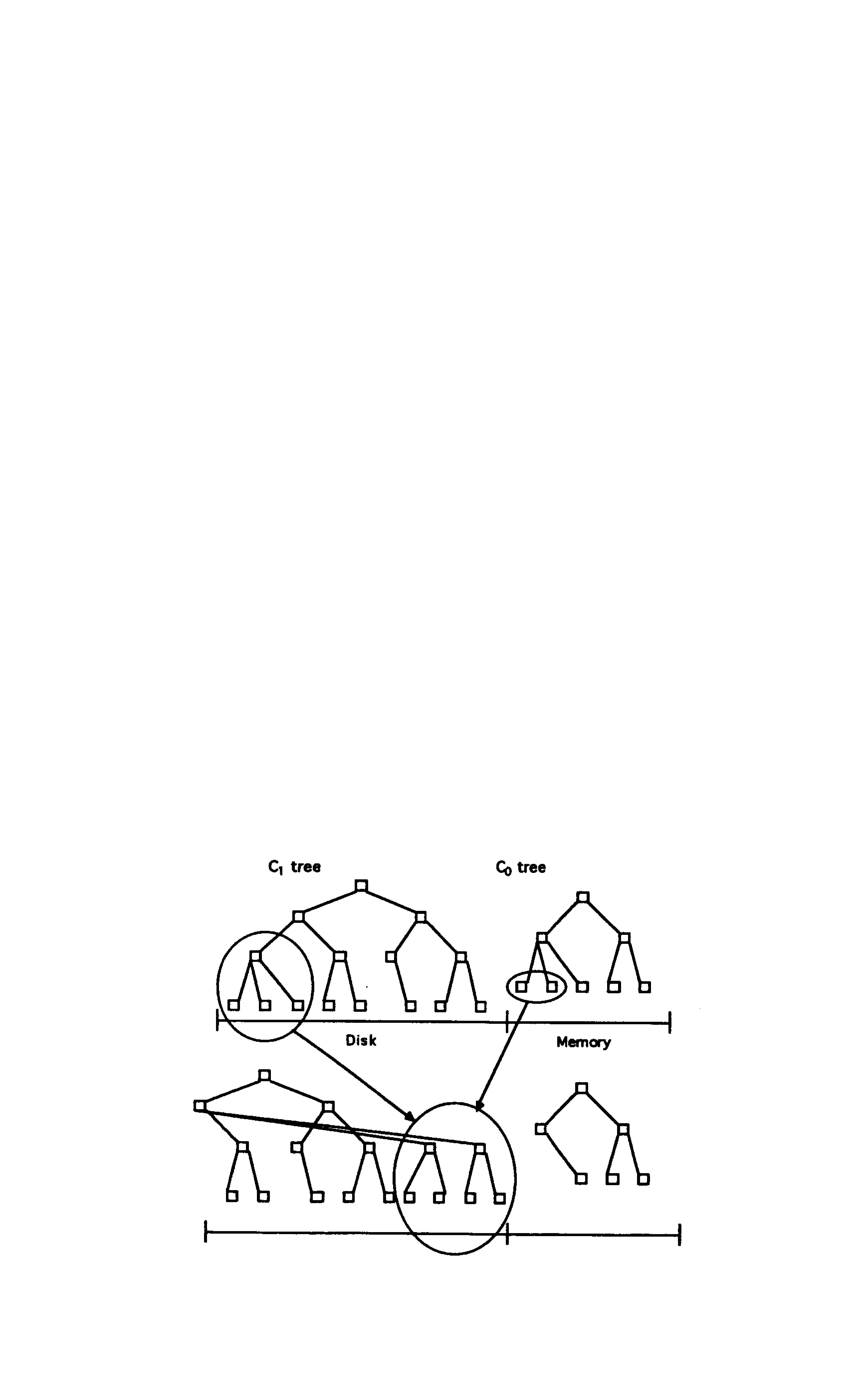
\includegraphics[scale=0.7]{figures/merge_LSM.pdf}
    \caption{Rolling merge\cite{LSMTree}}
    \label{fig:LSMMerge}
\end{figure}

\noindent
Delete operations in the Log-Structured Merge-tree is processed by first searching for the entry in $C_0$. If found it is removed, while if the entry is not present a \emph{delete node entry} is created and placed by index, noting an entry row to delete. This block is then sent through the levels by following the rolling merge method as is done with insertions, and if the entry is found it is deleted. Updates are handled by first deleting an entry and then inserting a new one.
\newline

\noindent
An important part of optimising the LSM-tree is to find the most suitable sizes for the different components. The size of the in-memory component $C_0$ can be costly if it is too big, but must be big enough to decrease the amount of I/O operations needed to move entries to disk. The ratio between the sizes of $C_0$ and $C_1$ is given by $1/M$, where \emph{M} is the average number of entries merged during the rolling merge process between the two. The LSM-tree was originally designed with magnetic hard drives in mind, using sequential writes to optimize the use of the disk arm. This is however also a good solution for solid state drives (SDDs), as there is not a big gap performance-wise between sequential and random writes. In addition, the use of out-of-place updates is well suited as SSDs are prone to wear-down\cite{LSMSDD}.

\subsection{Today's LSM-trees}
The structure of LSM-trees have evolved over time, and is now widely used by different NoSQL systems such as Cassandra\cite{Cassandra} and Bigtable\cite{Bigtable}. The basic structure of the LSM-tree used today is similar to the one described in 1996\cite{LSMTree}, but instead of merging higher levels into components in the lower levels, components are merged together into a new one instead\cite{LSMSurvey}. In addition to B+-trees, \emph{Sorted-String Tables} (SSTables) are often used as index structures. SSTables is made up of a list containing data blocks storing key-value pairs ordered by key, and an index block storing the key range for that list. 

\subsubsection{Merging policies}

The increase in number of components causes lower query performance, which is addressed by using merging methods to reduce them. \emph{Leveling} and \emph{Tiering} are two merge policies used in practice. Each policy organize disk components into logical levels or tiers which are sized after a ratio \emph{T}. In the leveling merge policy, there is only one component per level and each component is \emph{T} times larges than the component in the level above it. Entries from the upper level will therefore be merged multiple times with its sub-level, until the sub-level is full and then merged further down. The tiering merge policy has \emph{T} components per level. When a level is full, all of its components are merged together into a new component at the level below. The tiering merge policy is optimized for a high write-load, while the leveling merge policy is better performance-wise for query performance as the number of components to search is reduced\cite{LSMSurvey}. 

\subsubsection{Challenges}
With today's LSM-trees there are still areas that can be improved, as discussed by Luo and Carey\cite{LSMSurvey} \newline

\noindent
\textbf{Write amplification} is an issue as data has to be written multiple times when sending it through levels for merging. This can in the long run lead to wear-down of disk pages in SSDs. This is however improved with the use of the tiering merge policy as it has better write performance. Examples of this can be found in the WriteBuffer Tree\cite{WBTree}, LWC-Tree\cite{LWCTree1}\cite{LWCTree2} and PebblesDB\cite{PebblesDB}. They all use a partitioned tiering design with vertical grouping. There also exists other methods trying to reduce the write amplification, such as merge skipping which skips levels when merging data down through the levels\cite{SkipTree} and exploiting data skew by keeping track of hot and cold entries and only sending cold entries to disk\cite{TRIAD}. Keeping the hot entries in memory saves write operations as they can be written over directly. \newline

\noindent
\textbf{Merge operations} are an important part of LSM-trees, and can lead to buffer cache misses and write stalls when large merge operations are processed. Examples of improving the merge performance can be to check if a page from an SSTable overlaps with any of the pages in the SSTable it is to be merged with. If not, the resulting SSTable can contain pointers instead of having to read and write the pages during merge\cite{VTTree}. Another method is to use pipelining during the merging process, as it can be divided into three separate processes, where the merge operation is CPU-based. By doing this, the CPU is utilised in a more effective manner\cite{ZhangEtAl}. To avoid buffer cache misses, external servers can be used for large merge operations\cite{AhmadEtAl} or the old SSTable (before merge) can be stored in a buffer in the underlying level\cite{LSbMTree1}\cite{LSbMTree2}. This is however mainly effective on skewed workloads as storing cold pages additionally is not optimal. To minimize write stalls the write-throughput can be limited by only allowing a merge operation in a level to continue if the previous merge operation in that level has finished\cite{bLSM}. \newline

\noindent
\textbf{Hardware} has evolved since LSM-trees was first introduced. As LSM-trees was designed based on magnetic hard drives it is important to find better ways to utilize the new storage devices and their benefits. \newline

\noindent
\textbf{Special workloads} also have an effect on the structure of LSM-trees. The distribution can for example be a factor that should be taken into account when deciding the implementation. \newline

\noindent
\textbf{Auto-tuning} is mostly ways of optimizing the LSM-tree for the intended use. As explained in the RUM conjecture\cite{RUM}, access methods cannot be read- write and space-optimal at the same time. The different ways of tuning the LSM-tree can therefore be a great way to adapt to different workloads and in which ways they are handled. A challenge with auto-tuning is that there are many different aspects to tune, such as choosing the correct merge policy and finding the correct size ratio between components.
